\documentclass[12pt,fleqn]{article}\usepackage{../common}
\begin{document}
Orneklem Dagilimlari (Sampling Distributions)

$\frac{\bar{Y}-\mu}{\sigma / \sqrt{n}}$ ve $\frac{\bar{Y}-\mu}{S /
  \sqrt{n}}$ Karsilastirmasi

Diyelim ki normal olarak dagildigini bildigimiz bir nufustan $Y_1,..,Y_n$
rasgele orneklemini topladik, ve amacimiz bilinmeyen gercek $\mu$ hakkinda
bazi sonuclara varmak. Eger varyans $\sigma^2$ biliniyorsa, bu noktadan
sonra ne yapacagimiz gayet acik: daha once gordugumuz gibi bir karar kurali
ortaya cikartmak, ya da guven araligi hesaplamak cok kolay, ki bu
tekniklerin temelinde $Z = \frac{\bar{Y}-\mu}{\sigma / \sqrt{n}}$ dagiliminin standart normal $f_Z(z)$'ye 
yaklasmasi yatiyor. 

Fakat pratikte $\sigma^2$ genellikle bilinmez, o zaman nufus varyansinin
tahmin edicisi $S^2 = \frac{1}{n-1}\sum_{i=1}^n (Y_i-\bar{Y})^2$
kullanilir, ki bu maksimum olurluk tahmin edicisinin yansiz (unbiased)
versiyonu. Fakat buradaki onemli soru su: $\sigma^2$ yerine $S^2$ koyma Z
oranini nasil etkiler? Daha once buyuk orneklemler icin bir fark
olmadigindan bahsettik. Peki kucuk orneklemler icin? 

Kucuk $n$ icin bu iki oraninin birbirinden farkli oldugununun kesfi William
Sealy Gossett adli arastirmaciya ait. 1899'da Oxford'dan Kimya ve Matematik
bolumunden mezun olduktan sonra Gossey, Guiness adli sirkette calismaya
basladi. Urunlerin uzerinde yapacagi deneylerden aldigi veriler lojistik
bazi sebepler dolasisiyla cok azdi, ve ``gercek'' $\sigma^2$'nin bilinmesi
mumkun degildi. Cogu zaman $n$ 4 ya da 5'den bile az oluyordu. Bu gibi
durumlarla ugrasa ugrasa Gossey $\frac{\bar{Y}-\mu}{S / \sqrt{n}}$'nin
beklendigi gibi can egrisi $f_Z(z)$ seklinde degil, daha ``etekleri
kabarik'' baska bir dagilim gibi gozuktugunu farketti, yani sifirdan cok
kucuk ya da ondan cok buyuk oranlarin ihtimali cok dusuk degildi. 
 
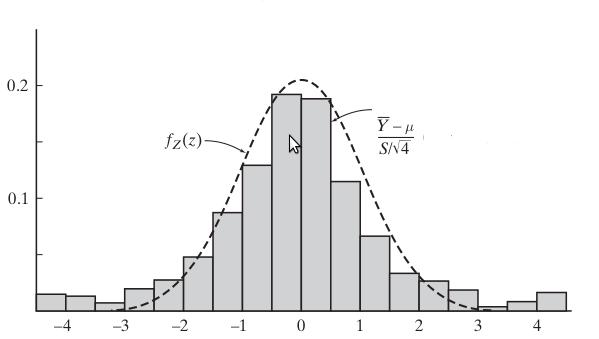
\includegraphics[height=5cm]{t1.png}

Ustteki histogram $S$ kullanarak hesaplanmistir, $n=4$ olmak uzere 500
orneklem uzerinden hesap yapilmistir. Iki dagilimin birbirinden uzaklastigi
goruluyor. 

Genel olarak olasilik dagilimlari iki buyuk kategori altina duser. Asagi
yukari bir duzine kadari gercek dunyadan alinabilecek her olcumu oldugu
haliyle iyi modelleme kabiliyetine sahiptir; mesela normal, binom, Poisson,
ustel dagilimlar gibi. Diger yandan daha az sayida (ama bir o kadar onemli)
dagilimlar $n$ tane rasgele degiskenin uzerinden hesaplanan {\em
  fonksiyonlarin} nasil davrandigini cok iyi modeller. Iste bu dagilimlara
orneklem dagilimlari ismi verilir ve tipik kullanim alanlari cikarsama
(inference) yapmaktir. 

Normal dagilimi her iki kategoriye de aittir. Hem ayri ayri olcumleri
modellemek, hem de $T = \frac{\bar{Y}-\mu}{\sigma / \sqrt{n}}$'in
olasiliksal davranisini modellemek icin kullanilir. Ikinci kullanimi normal
dagilimin bir orneklem dagilimi olarak kullanilmasina ornektir. 

Normal dagilimdan sonra en onemli uc orneklem dagilimi Ogrenci t Dagilimi,
chi kare dagilimi ve F dagilimidir. Son iki dagilim t oranini temsil eden
$f_T(t)$'yi, yani $T = \frac{\bar{Y}-\mu}{\sigma / \sqrt{n}}$'yi turetmek
icin gerekli.

Turetmek 

t Dagiliminin ispati icin su basamaklar gerekiyor; Once standart normal
rasgele degiskenlerin karelerinin toplaminin gamma dagilimin ozel bir hali
olan chi kare dagilimi oldugunu gostermek. Daha sonra normal dagilmis olan
bir nufustan alinan $n$ orneklemden elde edilen $\bar{Y}$ ve $S^2$'nin
birbirinden bagimsiz rasgele degiskenler oldugunu gostermek, ve
$\frac{n-1}{S^2}$'nin chi kare olarak dagildigini ispatlamak. Daha sonra
sira birbirinden bagimsiz iki chi kare yogunluk fonksiyonunun arasindaki
orani turetmeye gelecek, ki bu bir F dagilimidir. En son olarak $T^2
=(\frac{\bar{Y}-\mu}{S / \sqrt{n}})^2$ ifadesinin 
birbirinden bagimsiz iki chi kare dagiliminin orani oldugunu gostermek ki
$T^2$  ifadesi F dagiliminin ozel bir halidir.

Chi Kare, $\chi^2$ Dagilimi

Tanim

$Z_1, .. , Z_p$ bagimsiz standart Normal rasgele degiskenler ise, $U = \sum
_{ i=1}^{p} Z_p^2$ 
ki bu dagilima $p$ derecede serbestlige (degrees of freedom) olan chi kare
dagilimi (chi square distribution, yani $\chi^2$) ismi verilir.

Teori

$U$, $p$ derece serbestlige sahip bir $\chi^2$ dagilima sahip ise, ki yogunluk 

$$ f_U(u) = \frac{ 1}{\Gamma(\frac{p}{2}) 2^{p/2}} u^{(p/2) - 1} e^{-u/2
} $$

$$ u \ge 0 $$

formulune esittir. Ustteki yogunlugun $r=m/2$ ve $\lambda=1/2$ olan bir
Gamma dagilimi oldugu soylenebilir. Ispat icin [1].

F Dagilimi

Diyelim ki $U$ ve $V$ birbirinden bagimsiz, ve sirasiyla $m$ ve $n$ derece
serbestlige sahip iki chi kare dagilimi. O zaman $\frac{V/m}{U/m}$ olarak
hesaplanan yeni bir rasgele degiskenin dagilimi, $m,n$ derece serbestlige
sahip bir F dagilimi olarak ifade edilir.

Teori

Rasgele degisken $\frac{Z^2}{U/n}$, ki $U$ bir chi kare dagilimidir, 1,n
derece serbestlige sahip bir F dagilimina sahiptir. 

Ispati burada vermiyoruz.

Teori

$Y_1,..,Y_n$ ortalamasi $\mu$, varyansi $\sigma^2$ olan bir normal dagilimdan alinan $n$ 
orneklem olsun. O zaman 

a. $S^2$ ve $\bar{Y}$ birbirinden bagimsizdir

b. $\frac{(n-1)S^2}{\sigma^2} =
\frac{1}{\sigma^2}\sum_{i=1}^{n}(Y_i-\bar{Y})^2)$ hesabi $n-1$ derece
serbestlige sahip bir chi kare dagilimidir.

Ispat icin [1].

Nihayet  $\frac{\bar{Y}-\mu}{S / \sqrt{n}}$ ifadesinin yogunlugunu bulmak icin tum altyapiya sahibiz. 

Tanim

$Z$ bir standart normal rasgele degisken, $U$ ise $n$ derece serbestlikteki
bir chi kare rasgele degisken olsun. O zaman $n$ derece serbestligi olan
Ogrenci t orani (Student's t ratio)

$$ T_n = \frac{Z}{\sqrt{ \frac{U}{n}}} \mlabel{2} $$

olarak belirtilir.

Teori

$Y_1,..,Y_n$, bir $\mu,\sigma$ normal bir dagilimdan alinmis bir rasgele
orneklem olsun. O zaman 

$$ T_{n-1} = \frac{\bar{Y}-\mu}{S/\sqrt{n}}$$

$n-1$ serbestlik derecesine sahip bir t Dagilimidir. 

Ispat

$\frac{\bar{Y}-\mu}{S/\sqrt{n}}$ ifadesini su sekilde yazabiliriz, 

$$ \frac{\bar{Y}-\mu}{S/\sqrt{n}} =
\frac{\frac{\bar{Y}-\mu}{\sigma/\sqrt{n}} }
{\sqrt{\frac{(n-1)S^2}{\sigma^2(n-1)}}}
$$

Degil mi? Bolendeki $n-1$'ler birbirini iptal eder, ve $\sigma$ bolumdekini
iptal eder, ve nihai bolume $\sqrt{S^2}$ yani $S$ yerlestirilmis olur, ve
esitligin solundaki ifadeye erisiriz. Fakat bu donusturucu bolum ifadesi
sayesinde esitligin sag tarafinda yeni bir formule eristik; karekok ifadesi
icine bakarsak ustteki (b) teorisiyle uyumlu olarak
$\frac{(n-1)S^2}{\sigma^2}$ goruyoruz, ki bu ifade bir chi kare dagilimi.

Diger yandan esitligin sagindaki bolum kismi bir standart normal. Yani
(2)'de tarif edilen duruma erismis oluyoruz, ustteki ifade bu tanima gore
bir t Dagilimi. 


t Dagilimi (Student's t) 

$X$, $n$ derece bagimsizlikta $t$ dagilimina sahiptir, ve dagilimi

$$ 
f_T(t) = 
\frac
{
\Gamma(\frac{n+1}{2})
}
{
\sqrt{n\pi}\Gamma(\frac{n}{2})
\bigg(1+\frac{t^2}{n}\bigg)^{(n+1)/2}
}
 $$

Aslinda Normal dagilimi $t$ dagiliminin $v = \infty$ oldugu hale tekabul
eder. Cauchy dagilimi da $t$'nin ozel bir halidir, $n = 1$ halidir. Bu
durumda yogunluk fonksiyonu

$$ f(x)  = \frac{ 1}{\pi(1+ x^2)} $$

Bu formul hakikaten bir yogunluk mudur? Kontrol icin entegralini alalim, 

$$ \int _{ -\infty}^{\infty} f(x) dx = 
\frac{ 1}{\pi} \int _{ -\infty}^{\infty} \frac{ dx}{1 + x^2} 
 $$

Cogunlukla entegre edilen yerde  ``1 arti ya da eksi bir seyin karesi''
turunde  bir ifade gorulurse, yerine gecirme (subsitution) islemi
trigonometrik  olarak  yapilir. 

$$  x = \tan \theta, \theta = \arctan x $$

$$ 1 + x^2 = 1 + \tan^2\theta = \sec^2\theta$$

$$ dx / d\theta = \sec^2\theta $$

O zaman 

$$ =
\frac{ 1}{\pi} \int _{ -\infty}^{\infty} \frac{ dx}{1 + x^2}   =
\frac{ 1}{\pi} \int _{ -\infty}^{\infty}  \frac{ 1}{\sec^2\theta}\sec^2\theta d\theta = 
\frac{ 1}{\pi} \int _{ -\infty}^{\infty}  1 \ d\theta = 
 $$

$$ = 
\frac{ 1}{\pi} \theta | _{ -\infty}^{\infty}   = 
\frac{ 1}{\pi} [\arctan(\infty) - \arctan(-\infty)]
 $$

$$ =
\frac{ 1}{\pi} [\frac{ \pi}{2} - (-\frac{ \pi}{2}) ] = 1
 $$


Guven Araliklari, Testler

Daha once Z oranini temel alarak guven araliklari ya da hipotez testleri
olusturmustuk. Bu islemler icin standart normal dagilimin ust ve alt
yuzdelikleri hakkinda bazi bilgiler gerekmisti. Bu bilgiler bir tablodan
bakilan degerlerdi ya da istatistik yazilimimizda gerekli bir cagri ile
hemen bulunabiliyorlardi.

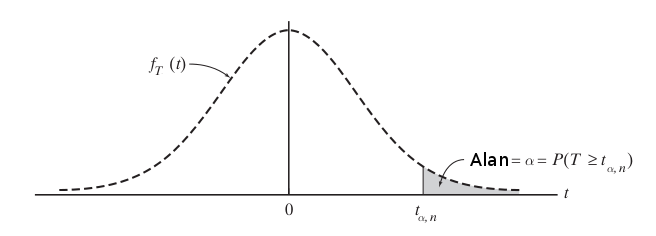
\includegraphics[height=4cm]{t2.png}

Ogrenci t'nin Z'ye gore farkli bir tarafi belli bir degeri bulmak icin iki
parametreye ihtiyac olmasi, bunlardan biri $\alpha$ digeri ise serbestlik
derecesi (degree of freedom -dof-). Standart normal icin tablo paylastik,
fakat t icin artik tablolarla ugrasmayacagiz, bilgisayar cagindayiz,
yazilim ile bu isi halledelim! 

Ornek

$T$ bir Ogrenci t dagilimi ise, ve serbestlik derecesi 3 ise, $\alpha=0.01$
icin icin $f_T(t)$'nin $100(1-\alpha)$ yuzdeligi nedir? Ustteki grafikteki
$t_{\alpha,n}$ notasyonundan hareketle $t_{0.01,3}$ degerini ariyoruz yani.

\begin{minted}[fontsize=\footnotesize]{python}
from scipy.stats.distributions import t
df = 3
print t.ppf(0.99,df)
print 1-t.cdf(4.541,df)
\end{minted}

\begin{verbatim}
4.5407028587
0.00999823806449
\end{verbatim}

Yani

$$ P(T_3 \ge 4.541) = 0.01 $$

$\frac{\bar{Y}-\mu}{S/\sqrt{n}}$ ifadesinin n-1 derece serbestlige sahip Ogrenci t dagilimina sahip 
oldugunu bilmek alttaki ifadeyi mumkun kilar, 

$$ P \bigg(
-t_{\alpha/2,n-1} \le
\frac{\bar{Y}-\mu}{S/\sqrt{n}} \le 
t_{\alpha/2,n-1}
\bigg) = 1-\alpha
 $$

Bu ifadeyi daha once standart normal icin yaptigimiz gibi tekrar
duzenlersek,

$$ P \bigg(
\bar{Y}-t_{\alpha/2,n-1}\frac{S}{\sqrt{n}} \le
\mu \le 
\bar{Y}+t_{\alpha/2,n-1}\frac{S}{\sqrt{n}}
\bigg) = 1-\alpha
$$

Tabii, $Y_i$'larin normal dagilimdan gelmis olmasi lazim. Bunun sonucunda
gercek veri temel alinarak hesaplanacak $S$ ve $\bar{Y}$ bize $\mu$ icin
bir $100(1-\alpha)$ guven araligi verecektir. 


Tek Orneklem t Testi (The One-Sample t test)

Bu test verinin bir $N(\mu,\sigma)$ Normal dagilimindan geldigini farzeder,
test etmek istedigimiz hipotez / karsilastirma $\mu = \mu_0$. Ayrica
$\sigma$ bilinmiyor, ki Ogrenci t dagilimindan bahsetmemizin ana sebebi
buydu zaten, o zaman hipotez testine Tek Orneklem t Testi adi verilir.

Ornek

Alttaki veride bir grup hanimin ne kadar kalori tukettigi
kayitlanmis. Acaba bu hanimlarin aldigi enerji tavsiye edilen 7725'ten ne
kadar sapmistir?

\begin{minted}[fontsize=\footnotesize]{python}
daily_intake = np.array([5260,5470,5640,6180,6390,6515, 6805,7515,7515,8230,8770])
\end{minted}

t degerini $\frac{\bar{y}-\mu_o}{s/\sqrt{n}}$ olarak hesaplayacagiz, ki $\mu_0=7725$ olacak. 

\begin{minted}[fontsize=\footnotesize]{python}
from scipy.stats.distributions import t
df = len(daily_intake)-1 # serbestlik derecesi
mu0 = 7725
ybar = np.mean(daily_intake)
s = np.std(daily_intake)
tval = (ybar-mu0)/(s/np.sqrt(len(daily_intake)))
print 'tval',tval
print 'sol',t.ppf(0.025,df)
print 'sag',t.ppf(0.975,df)
\end{minted}

\begin{verbatim}
tval -2.95843181751
sol -2.22813885196
sag 2.22813885196
\end{verbatim}

Sonuc t degeri soldaki esik degerinden kucuk cikti demek ki \%95
seviyesinde hipotezi reddetmek gerekir. Ayni hesabi kutuphane cagrisi ile
yaparsak,

\begin{minted}[fontsize=\footnotesize]{python}
from scipy.stats import ttest_1samp
t_statistic, p_value = ttest_1samp(daily_intake, 7725)
print "one-sample t-test", p_value
\end{minted}

\begin{verbatim}
one-sample t-test 0.0181372351761
\end{verbatim}

Sonuc \verb!p_value! \verb!0.05!'ten kucuk cikti yani yuzde 5 onemliligini
(significance) baz aldik bu durumda veri hipotezden onemli derecede
(significantly) uzakta. Demek ki ortalamanin 7725 oldugu hipotezini
reddetmemiz gerekiyor.

Testi iki orneklemli kullanalim, gruplar 0/1 degerleri ile
isaretlendi, ve test etmek istedigimiz iki grubun ortalamasinin (mean)
ayni oldugu hipotezini test etmek. t-test bu arada varyansin ayni
oldugunu farzeder.

\begin{minted}[fontsize=\footnotesize]{python}
energ = np.array([
[9.21, 0],[7.53, 1],
[7.48, 1],[8.08, 1],
[8.09, 1],[10.15, 1],
[8.40, 1],[10.88, 1],
[6.13, 1],[7.90, 1],
[11.51, 0],[12.79, 0],
[7.05, 1],[11.85, 0],
[9.97, 0],[7.48, 1],
[8.79, 0],[9.69, 0],
[9.68, 0],[7.58, 1],
[9.19, 0],[8.11, 1]])
group1 = energ[energ[:, 1] == 0][:, 0]
group2 = energ[energ[:, 1] == 1][:, 0]
t_statistic, p_value = ttest_ind(group1, group2)
print "two-sample t-test", p_value
\end{minted}

\begin{verbatim}
two-sample t-test 0.00079899821117
\end{verbatim}

$p$ degeri < 0.05 yani iki grubun ortalamasi ayni degildir. Ayni oldugu
hipotezi reddedildi.

Eslemeli t-Test (Paired t-test)

Eslemeli testler ayni deneysel birimin olcumu alindigi zaman
kullanilabilir, yani olcum alinan ayni grupta, deney sonrasi deneyin
etki edip etmedigi test edilebilir. Bunun icin ayni olcum deney
sonrasi bir daha alinir ve "farklarin ortalamasinin sifir oldugu"
hipotezi test edilebilir. Altta bir grup hastanin deney oncesi ve
sonrasi ne kadar yiyecek tukettigi listelenmis. 

\begin{minted}[fontsize=\footnotesize]{python}
intake = np.array([
[5260, 3910],[5470, 4220],
[5640, 3885],[6180, 5160],
[6390, 5645],[6515, 4680],
[6805, 5265],[7515, 5975],
[7515, 6790],[8230, 6900],
[8770, 7335],
])
pre = intake[:, 0]
post = intake[:, 1]
t_statistic, p_value = ttest_1samp(post - pre, 0)
print "paired t-test", p_value
\end{minted}

\begin{verbatim}
paired t-test 3.05902094293e-07
\end{verbatim}

Kaynaklar

Larsen, {\em Introduction to Mathematical Statistics and Its Applications}

\end{document}
